\begin{figure}[!h]
  \centerline{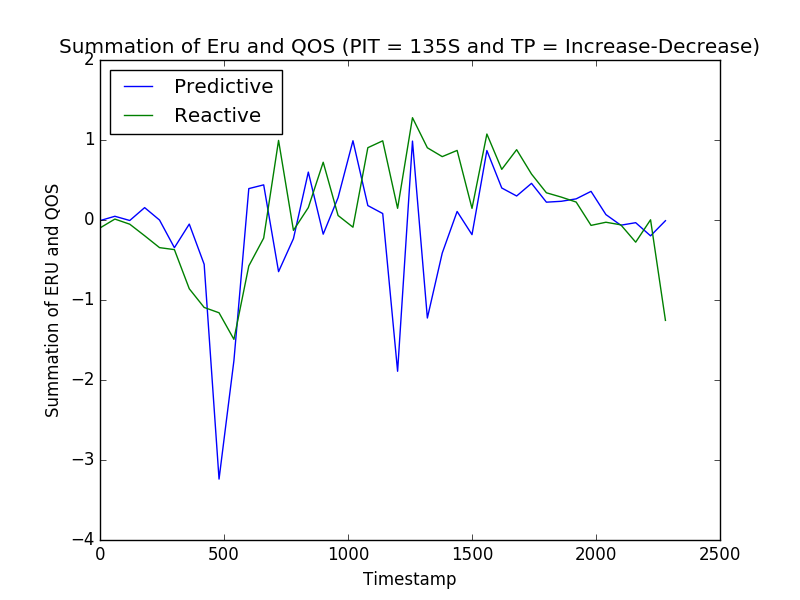
\includegraphics[scale=.75]{graph_135s_increase-decrease.png}}
  \caption{The graph for 135s, increase-decrease}
  \label{fig:135s-increase-decrease}
\end{figure}

\begin{table}[htbp]
  \centering
  \caption{Difference in Predictive and Reactive Auto-scaling for 135s, increase-decrease}
  \label{tab:135s-increase-decrease}
\begin{tabular}{l c}\hline\hline
    \multicolumn{1}{c}{\textbf{Measure}} & \textbf{Value} \\ \hline
     p-value & 0.591 \\
     z-score & -.230 \\
     std\_dev & .803 \\
     mean & -.185
  \end{tabular}
\end{table}

Figure \ref{fig:135s-increase-decrease} contains a graph
showing predictive and reactive auto-scaling's different
summations of efficient resource utilization and quality of service over the
course of the forty minute trial. Additionally, Table
\ref{tab:135s-increase-decrease} shows summary statistics for predictive
auto-scaling's summation of ERU and QOS minus reactive auto-scaling's summation
of ERU and QOS for corresponding intervals.

As can be seen from the summary statistics, with a p-value of .591 we are not
able to reject our null hypothesis that there is no difference between the
summation of ERU and QOS for predictive and reactive auto-scaling in favor of
our alternative hypothesis that there is a positive difference in the summation
of ERU and QOS for predictive and reactive auto-scaling. Still, upon a closer
examination of the graph, we can see that predictive auto-scaling did outperform
reactive auto-scaling at times, just not necessarily consistently. As can be
seen from the graph, predictive and reactive auto-scaling follow somewhat
similar patterns, just with reactive auto-scaling shifted to the right. In
short, this means predictive auto-scaling realizes the benefits of auto-scaling
sooner than reactive auto-scaling. However, because Kubernetes imposes a time
limit between auto-scales, reactive auto-scaling is often able to scale under
heavier traffic, thus increasing its impact. Still, in conjunction with our goal
of providing options, predictive auto-scaling is useful with respect to
the increase-decrease traffic pattern when we want to be sure to respond
positively to initial increases in traffic, and accept that such an initial
response may have slightly less optimal ramifications later.
